\RequirePackage{luatex85}
\documentclass[tikz]{standalone}
% Default preamble
\usepackage{pgfplots}
\pgfplotsset{compat=newest}
\usepgfplotslibrary{groupplots}
\usepgfplotslibrary{polar}
\usepgfplotslibrary{smithchart}
\usepgfplotslibrary{statistics}
\usepgfplotslibrary{dateplot}
\usepgfplotslibrary{ternary}
\begin{document}
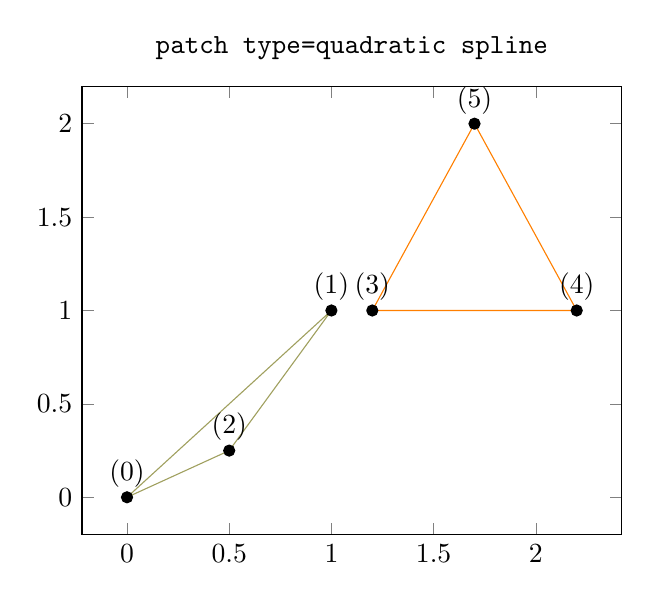
\begin{tikzpicture}
\begin{axis}[nodes near coords={(\coordindex)}, title={\texttt{patch type=quadratic spline}}]
    \addplot[mark={*}, patch, mesh]
        coordinates {
            (0,0)
            (1,1)
            (0.5,0.25)
            (1.2,1)
            (2.2,1)
            (1.7,2)
        }
        ;
\end{axis}
\end{tikzpicture}
\end{document}
